\documentclass[letterpaper,11pt]{article}

\usepackage[letterpaper, margin=0.75in]{geometry}
\usepackage{titlesec}
\usepackage[document]{ragged2e}
\usepackage{gensymb}
\usepackage{textcomp}
\usepackage{graphicx}
\usepackage{float}
\usepackage{wrapfig}


\setlength{\parskip}{1em}

\DeclareGraphicsExtensions{.jpg,.JPG}

\newcommand*{\TitleFont}{
      \usefont{\encodingdefault}{\rmdefault}{b}{n}
      \fontsize{12}{20}
      \selectfont}

\newcommand\blankpage{%
    \null
    \thispagestyle{empty}%
    %\addtocounter{page}{-1}%
    \newpage}
      
\begin{document}

% generates the title
%\maketitle
\begin{center}
\TitleFont AIT Measurement Standard Operating Procedure\newline
\TitleFont Last modified on: \today \hspace{1mm} by Mark Redd \newline
\end{center}

\titleformat{\section}
  {\normalfont\fontsize{12}{15}\bfseries}{\thesection}{1em}{}

\begin{itemize}
\item \textbf{NOTICE: Lab policy requires that any person performing 
    AIT measurements must have done the following before performing any 
    experimental work:}
    
    \begin{itemize}
    \item \textbf{Complete pertinent laboratory safety training 
    \item Read this SOP in its entirety
    \item Become familiar with all the experimental steps outlined in this SOP
    \item Sign and Date the AIT SOP Signatures Sheet}
    \end {itemize}
\end{itemize}
%\renewcommand{\baselinestretch}{.75}\normalsize
\tableofcontents    % insert the table of contents
%\renewcommand{\baselinestretch}{1.0}\normalsize
%\tableofcontents 

\newpage

\section{Introduction}
This SOP outlines the established procedure for performing autoignition 
temperature (AIT) experiments in Dr. Wilding's laboratory (CB 343A), including 
detailed instructions on how to perform experiments and corresponding safety 
protocols. As such, lab policy requires every person working on AIT to have read
and become familiar with the most updated version of this document and affirm 
this by signing the AIT SOP Signatures Sheet.

This document is intended to outline experimental procedures that conform to
ASTM Standard E659. If any part of the experimental procedure violates the 
standard, that part should be changed promptly to conform to established 
guidelines in ASTM Standard E659. The only exception to this rule is when 
conforming to the standard would present a significant hazard or risk.

This document will be updated continually as changes to the process are made or 
improvements are found. If you find an error in this document or have a 
suggestion to improve it please contact the last person who modified it to 
submit your proposed changes.

\section{Safety and Hazard Mitigation}
Prior to performing experimental work, all researchers should be familiar with
this section, which outlines the hazards considered in these 
experiments as well as the steps taken to mitigate them. While reading the 
remainder of this SOP, researchers should note which steps in the procedure 
control for these hazards. If there are hazards that could be better mitigated, 
researchers should propose appropriate changes to the SOP.

There are three primary hazards that exist in this experiment. These hazards are
listed below with corresponding general protocols that have been implemented to 
mitigate them.

\begin{itemize}
\item Electrical shock from furnace, heat gun, computer or other sources
    \begin{itemize}
    \item Researchers will receive corresponding training about safe use of 
        electrical equipment and follow established standards for electrical 
        safety including lockout-tagout protocol
    \end{itemize}

\item Exposure to toxic chemicals via skin or eye contact, inhalation or 
    ingestion
    \begin{itemize}
    \item Researchers will receive corresponding training about safe handling of
        chemicals
    \item Researchers will use appropriate PPE when handling any chemical based 
        on recommendations from the corresponding SDS and lab policy
    \item All handling of volatile chemicals will take place inside one of the 
    ventilated hoods in the lab
    \item As per ASTM Standard E659, small amounts of compound will be used in 
        any one experiment (Maximum amounts for any one experiment are limited 
        to 1 milliliter for liquids and 1 gram for solids and gases)
    \end{itemize}

\item Fire or explosion of flammable chemicals
    \begin{itemize}
    \item Researchers will receive corresponding training about fire and 
        explosion safety and prevention
    \item Experiments will take place in a ventilated hood
    \item A fire extinguisher is available in the lab in the event of a small 
        fire
    \item As per ASTM Standard E659, small amounts of compound will be used in 
        any one experiment (Maximum amounts for any one experiment are limited 
        to 1 milliliter for liquids and 1 gram for solids and gases)
    \end{itemize}  

\end{itemize}

\newpage
 
\section{Experimental Setup and Maintenance}
    \subsection{Flask and Lid}
    \begin{itemize}
    \item \textbf{Latex or nitrile gloves and safety glasses are 
            required while working with the flask/lid assembly}
    \item The flask in the furnace must be exchanged for a clean flask in the 
        following situations:
        \begin{itemize}
        \item The next experiment will be for a different compound
        \item The next experiment will be for a new container of the same 
            compound
        \item There is reason to suspect that the flask has become 
            contaminated or substantially dirty
        \item The flask has been used for 10 runs without being cleaned
        \item Once the AIT has been found for a compound, the final measurements
            should be repeated with a clean flask to verify the results
        \end{itemize}
    
    \item Disassembling the Flask and Lid
        \begin{itemize}
        \item \textbf{The furnace may be too hot to open for several hours after
             an experiment}
        \item Unplug the thermocouples from the furnace
        \item Once the furnace is cool, remove flask/lid assembly
            \begin{itemize}
            \item Loosen (do NOT remove) the nut that secures the bracket and 
                the rubber hose to the top of the furnace with a wrench
            \item Move the bracket out of the way and remove Thermocouple 4 
                (along with the rubber hose) from the top of the furnace
            \item Move the mirror out of the way to allow the flask/lid assembly
                to come out
            \item Grip the assembly with both hands by the screws on top and 
                pull directly upward
            \item \textbf{NOTE: The flask/lid assembly is heavy and pulling it  
                out can be awkward. Please ask someone to help you remove it 
                if you are at all unsure about removing the assembly}
            \item The flask/lid assembly should easily come out of the furnace 
                without catching on anything
            \end{itemize}
        
        \item \textbf{Carefully} set the assembly on a table or other stable 
            surface with the flask on top (See Figure \ref{fig:f_lid_done})
        \item Ensure the bracket screw is loose
        \item Remove the circular spring from its groove and slide the ceramic
            halves of the lid apart sufficiently to allow the flask to be 
            removed
        \item Remove flask from lid assembly and  remove all of the aluminum 
            foil and thermocouples from the flask
        \item Discard the used aluminum foil in a normal trash can and set 
            aside the thermocouples in the hood or on a surface where they will
            not catch on anything or become damaged
        \item \textbf{Always store bulb flasks on the drying rack above the sink 
            or appropriately secured to a ring stand} (see "Flask Cleaning"
             below)
        \end{itemize}

\newpage      
    \item Assembling the Flask and Lid 
        \begin{itemize}
        \item Use the figures in this section as a reference when putting 
            together the assembly
        
        \item Use a \textbf{clean}, 500 ml, round bottom, long neck, bulb flask 
            (PYREX\textsuperscript{\textcopyright} 500mL Long Neck Boiling 
            Flask, Round Bottom, Tooled Mouth, Product No.: 4280-500 from Corning Inc.)
        \item If dirty, wash out the flask using soap and water and dry as much 
            as possible (see "Flask Cleaning" below); be sure to rinse
            thoroughly
                \begin{itemize}
                \item Any leftover water will boil away when the furnace heats 
                up and before any measurements are taken
                \end{itemize}        
        \item Wrap entire flask in aluminum foil with thermocouples at the 
            bottom, side and top of the round part of the flask (thermocouples 
            should be touching the glass directly) (Refer to Figure 
            \ref{fig:wrap})
                \begin{itemize}
                \item NOTE: The more reflective side of the foil should always 
                    be facing inward
                \item Start by getting a long strip of aluminum foil (12" long 
                    or so)
                \item Use a utility knife to poke a hole near the middle of 
                    the foil and insert thermocouple 3 through the foil so the 
                    bead sits at the bottom of the flask and then wrap the foil 
                    around the bottom (1 and 2)
                \item Slide thermocouple 2 down to the approximate 
                    middle/equator of the flask between the flask and foil and 
                    use a second piece of foil to wrap further up the flask, 
                    ensuring the thermocouple wires run parallel up the side of 
                    the flask (3)
                \item Place thermocouple 1 at the top of the bulb of the flask 
                    (not on the neck of the flask) and use a third piece of foil
                     to wrap around the top starting at the middle (4)
                \item Add an additional layer of foil around  the flask so the 
                    wires are covered and run parallel when wrapping is finished
                    (5)
                \item Wrap additional foil around the neck of the flask to cover 
                    it completely and secure flask in lid assembly
                \item The thermocouple wires should emerge from the foil 
                    covering near the top (but not at the top) of the flask 
                    neck, allowing them to run between the two ceramic halves of
                    the lid assembly (6)
                \end{itemize}

\begin{figure}[H]
\centering
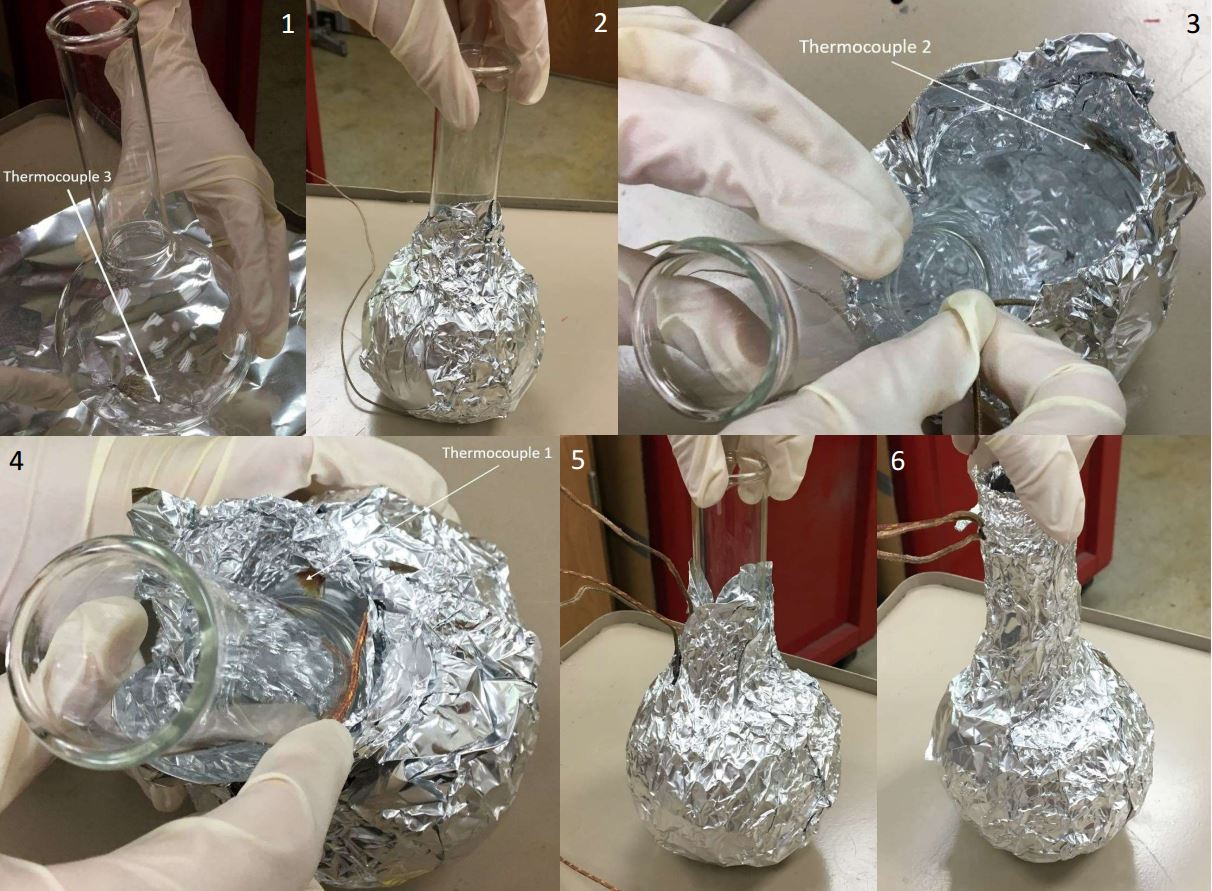
\includegraphics[width=1\textwidth]{wrap.jpg}
\caption{Steps for wrapping the flask in foil}
\label{fig:wrap}
\end{figure}

        \item Loosen the nut on top of the lid assembly and slide the 
            corresponding half of the ceramic part of the lid assembly out
        \item Fit the neck of the flask in the center hole of the ceramic lid 
            assembly with the lip of the flask fitting into the groove at the 
            base of the center hole on both sides
        \item Guide the thermocouple wires in the gap between the two ceramic 
            halves so they are out of the way when the flask/lid assembly is 
            inserted into the furnace
        \item Slide the loose half of the ceramic back in to be snug 
            around the flask neck and tighten the nut on the top to hold it
            in position
                \begin{itemize}
                \item The two halves nearest to the top of the assembly should 
                    meet or very nearly meet; if they don't then some 
                    foil should be removed from the neck of the flask
                \item Use a circular spring to help hold the halves together
                \end{itemize}
        
        \item Make a "donut" of foil wrapped around the neck of the flask that 
            will rest up against the bottom of the lid assembly
        \item Slide the foil "donut" up so and press it so it is flush against 
            the ceramic and restricts air flow around the opening
        \item Carefully turn the flask/lid assembly over making sure the flask 
            doesn't fall out
                \begin{itemize}
                \item \textbf{Do this over a table or close to a level surface 
                    to avoid accidental breaking of the flask}
                \item The flask will fit into the lid assembly somewhat loosely, 
                    but it shouldn't fall out
                \item If the flask falls out, remove it and add more foil 
                around the neck
                \end{itemize}
         
\begin{figure}[H]
\centering
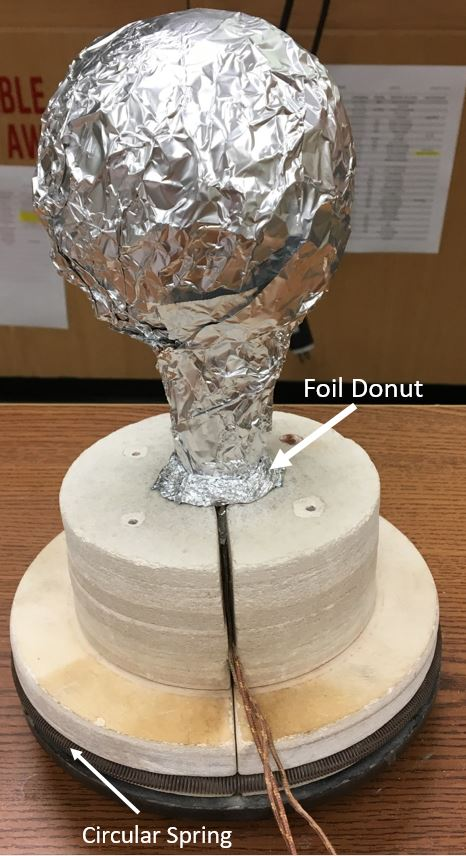
\includegraphics[width=.45\textwidth]{insert_in_lid_w_donut.jpg}
\caption{Final state of the flask/lid assembly}
\label{fig:f_lid_done}
\end{figure}
        
        \item See Figure \ref{fig:f_lid_done} for the final flask/lid
            assembly before insertion into the furnace
        \item Place the prepared flask/lid assembly into the furnace by gripping
            the assembly with both hands by the screws on top and slowly 
            lowering the assembly into place
        \item Turn the flask/lid assembly so the thermocouple wires point away 
            from where researchers will be working
        \item Insert flask interior thermocouple (\#4) carefully down the flask 
            neck, making sure it goes straight in and the bead doesn't get 
            caught anywhere
                \begin{itemize}
                \item The bead of Thermocouple 4 should be suspended in the 
                    approximate center of the flask, not be touching any part
                \item The wire of Thermocouple 4 should run up the edge of the 
                    neck and not the middle to allow compound to be injected 
                    without making contact with the thermocouple
                \item Use the bracket on one of the two screws on top of the 
                    lid to secure the rubber hose holding the thermocouple
                    in place
                \item Tighten the nut on the bracket hand tight and then give a 
                    half turn with a wrench to secure the nut (See Figure 
                    \ref{fig:wrench_tight})
                \end{itemize}

\begin{figure}[H]
\centering
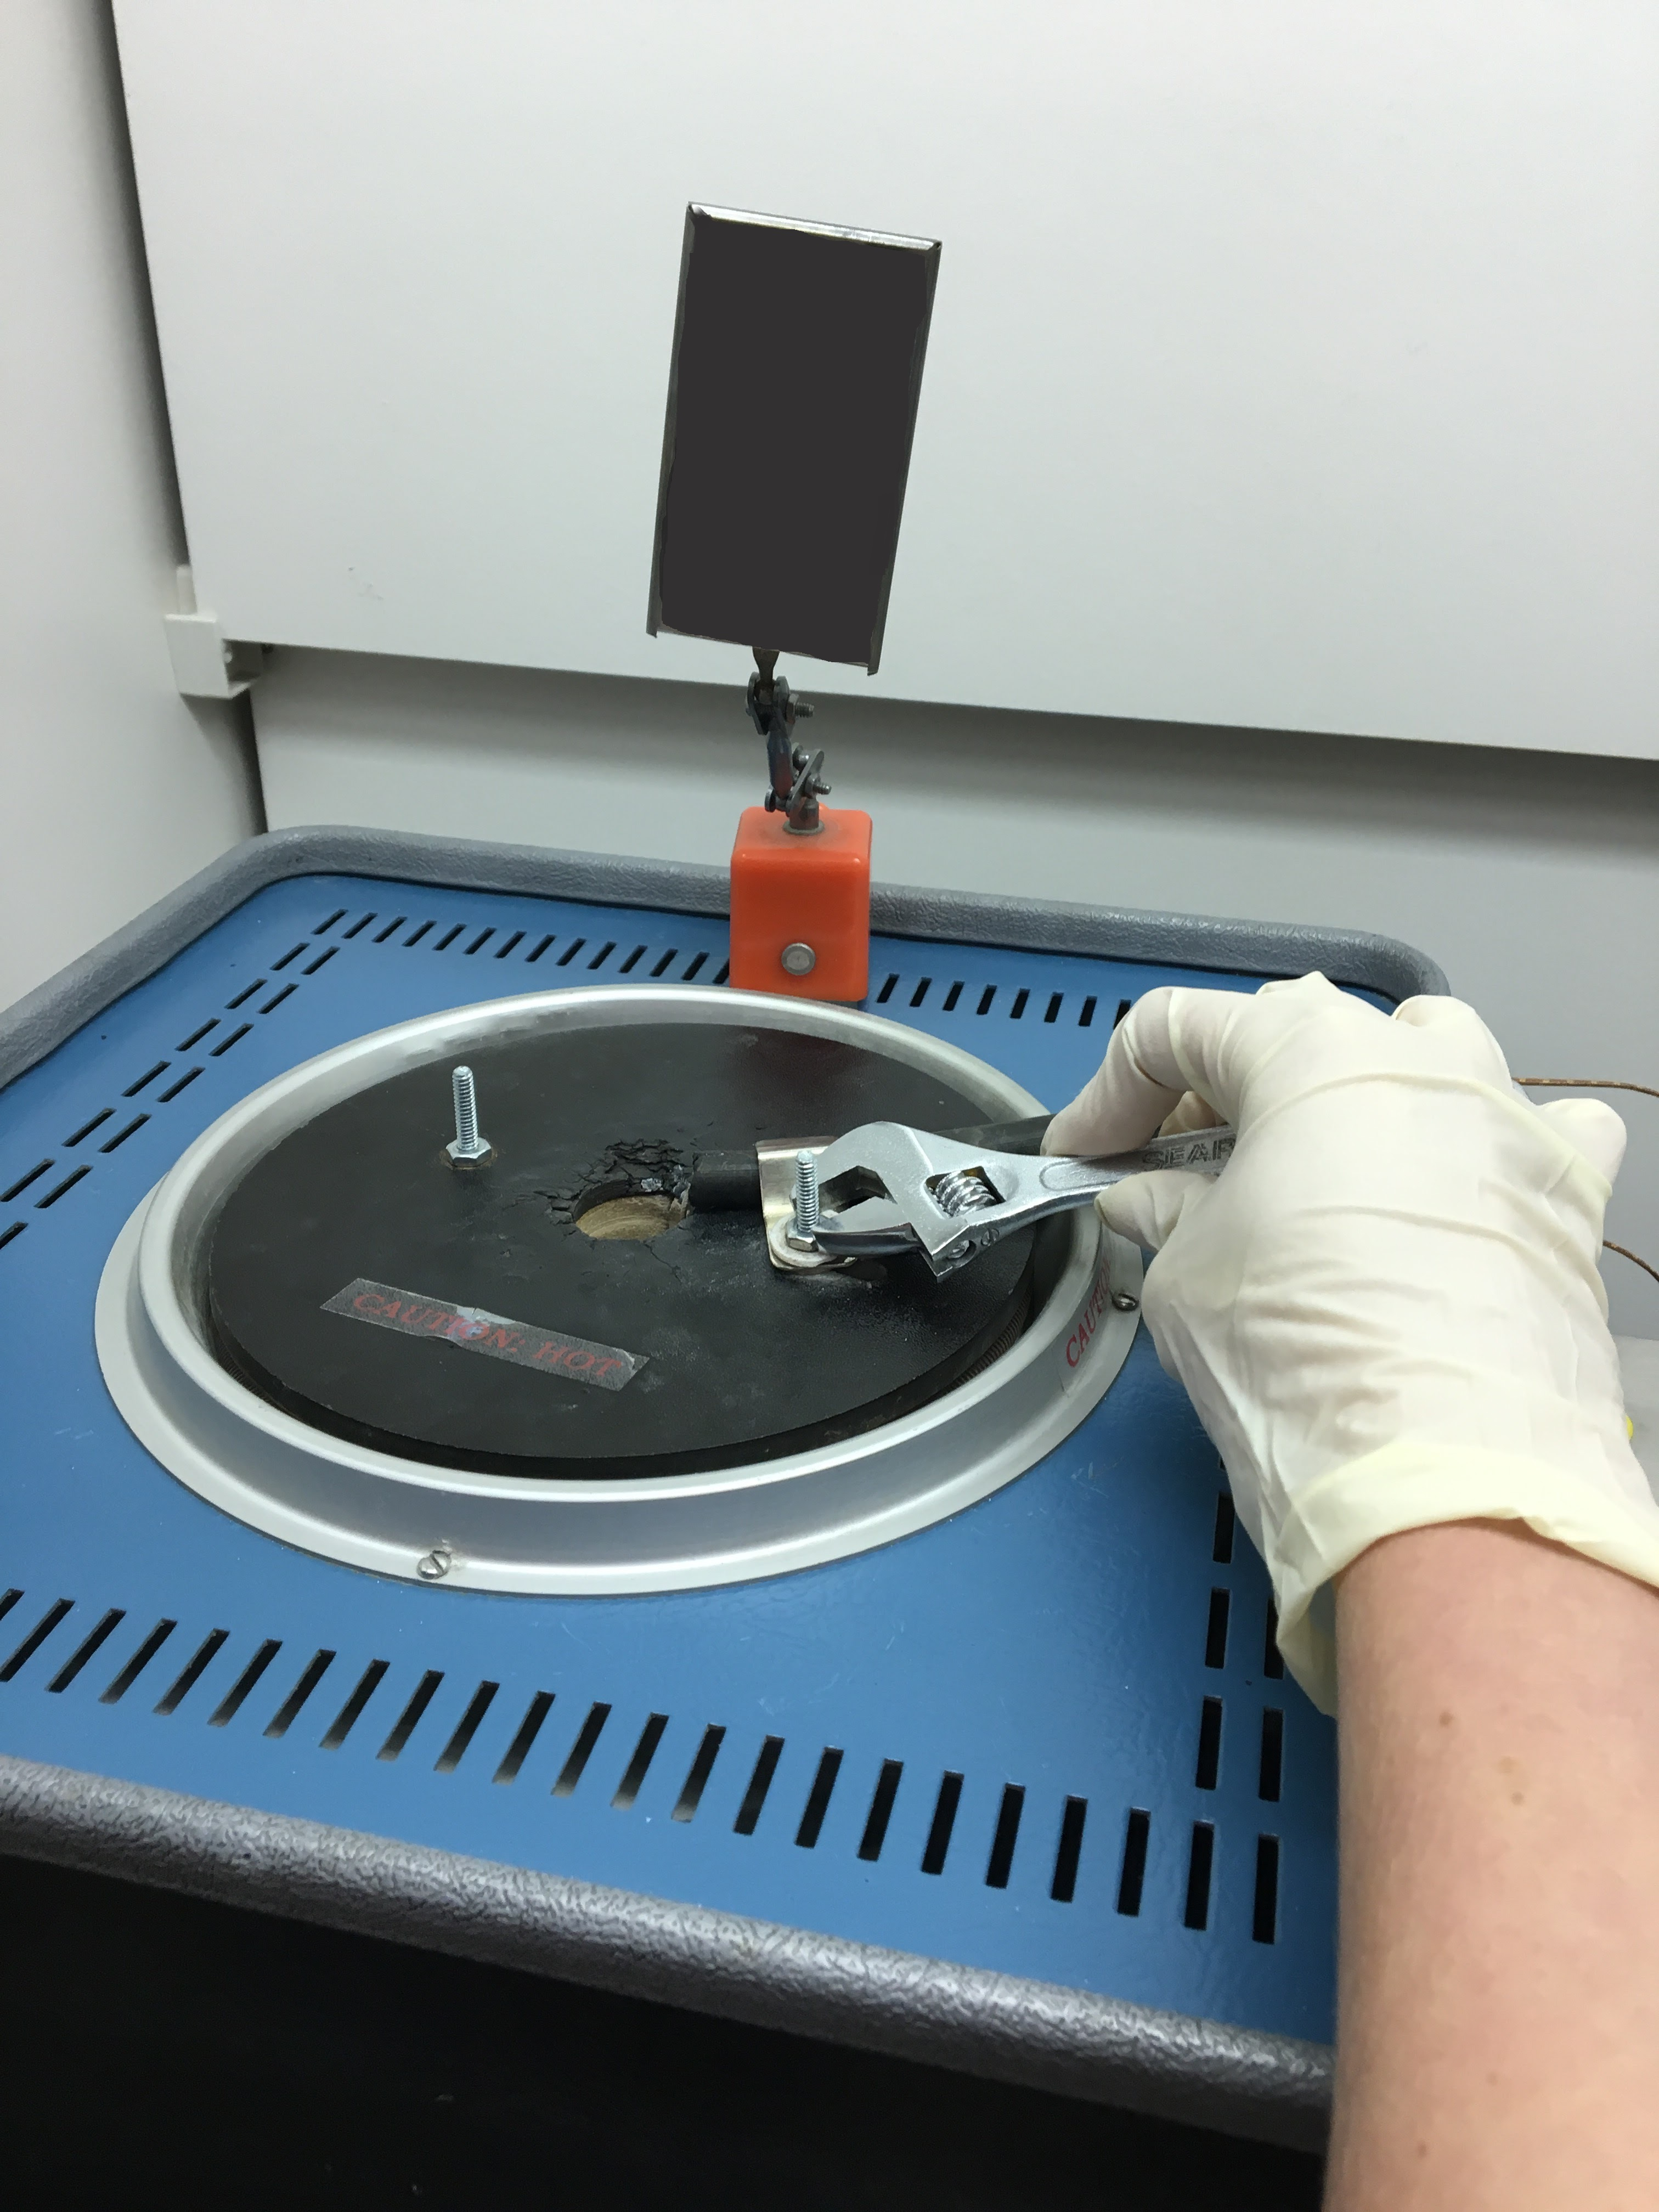
\includegraphics[width=.35\textwidth]{top_of_furnace_w_wrench.jpg}
\caption{Position thermocouple 4 with the rubber hose and tighten}
\label{fig:wrench_tight}
\end{figure}

        \item Connect the thermocouples to the TA-DA
        \item The final setup should resemble Figure \ref{fig:in_furnace}
        \end{itemize}
    
\begin{figure}[H]
\centering
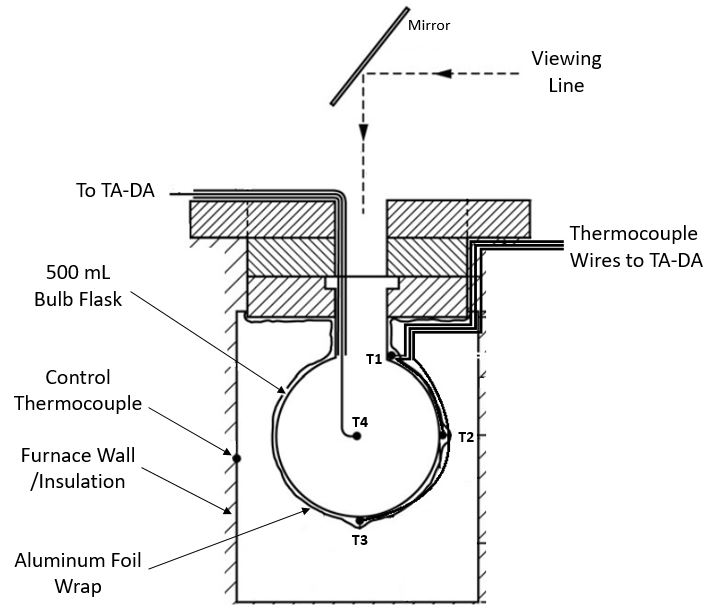
\includegraphics[width=.65\textwidth]{Furnace_diagram_mod.jpg}
\caption{Diagram of the furnace when assembled}
\label{fig:in_furnace}
\end{figure}

    \item Flask Cleaning \newline
        For consistent experimental results, flasks must be as clean as possible
        (See Figure \ref{fig:clean_dirty}). Dirty flasks can terminate radical 
        reactions and artificially raise the AIT. To ensure flasks are as clean 
        as possible before use, the following steps are required for flask 
        cleaning:
        \begin{itemize}
        \item Always begin by soaking the inside of the flask with soapy water 
            for 12 - 24 hours, regardless of how dirty it is
        \item While soaking, the flask should always be secured to a ring stand
        \item Wash out flask with soap and water, scrubbing the inside with 
            tube brushes
        \item For difficult stains, soak the flask inside with soapy water for 
            another 24 hours or longer if needed 
            \begin{itemize}
            \item During this process, scrub the inside and replace the 
                soapy water on a regular basis (generally every 12 - 24 hours)
            \end{itemize}
        
        \item Once all stains have been eradicated from the inside of the flask
            and the flask has been scrubbed in soapy water, rinse the inside and
            outside of the flask thoroughly
            \begin{itemize}
            \item Using hot water for rinsing is preferred but not required
            \item Rinse with tap water a minimum of 3 times, filling the flask
                with water, agitating the water for about 10 seconds, and then 
                dumping the water
            \item Repeat this process with distilled water available from the 
                smaller tap on the Northeast corner of the lab sink
            \end{itemize}
        
        \item If hard water spots or salt deposits appear on the inside of the 
            flask, rinse the inside of the flask with a small amount of vinegar
            to remove the deposits and repeat the rinse procedure above
        \item Once the flask has been cleaned and rinsed thoroughly, place the 
            clean flask on the drying rack over the sink
        \end{itemize}        
    \end{itemize}

\begin{figure}[H]
\centering
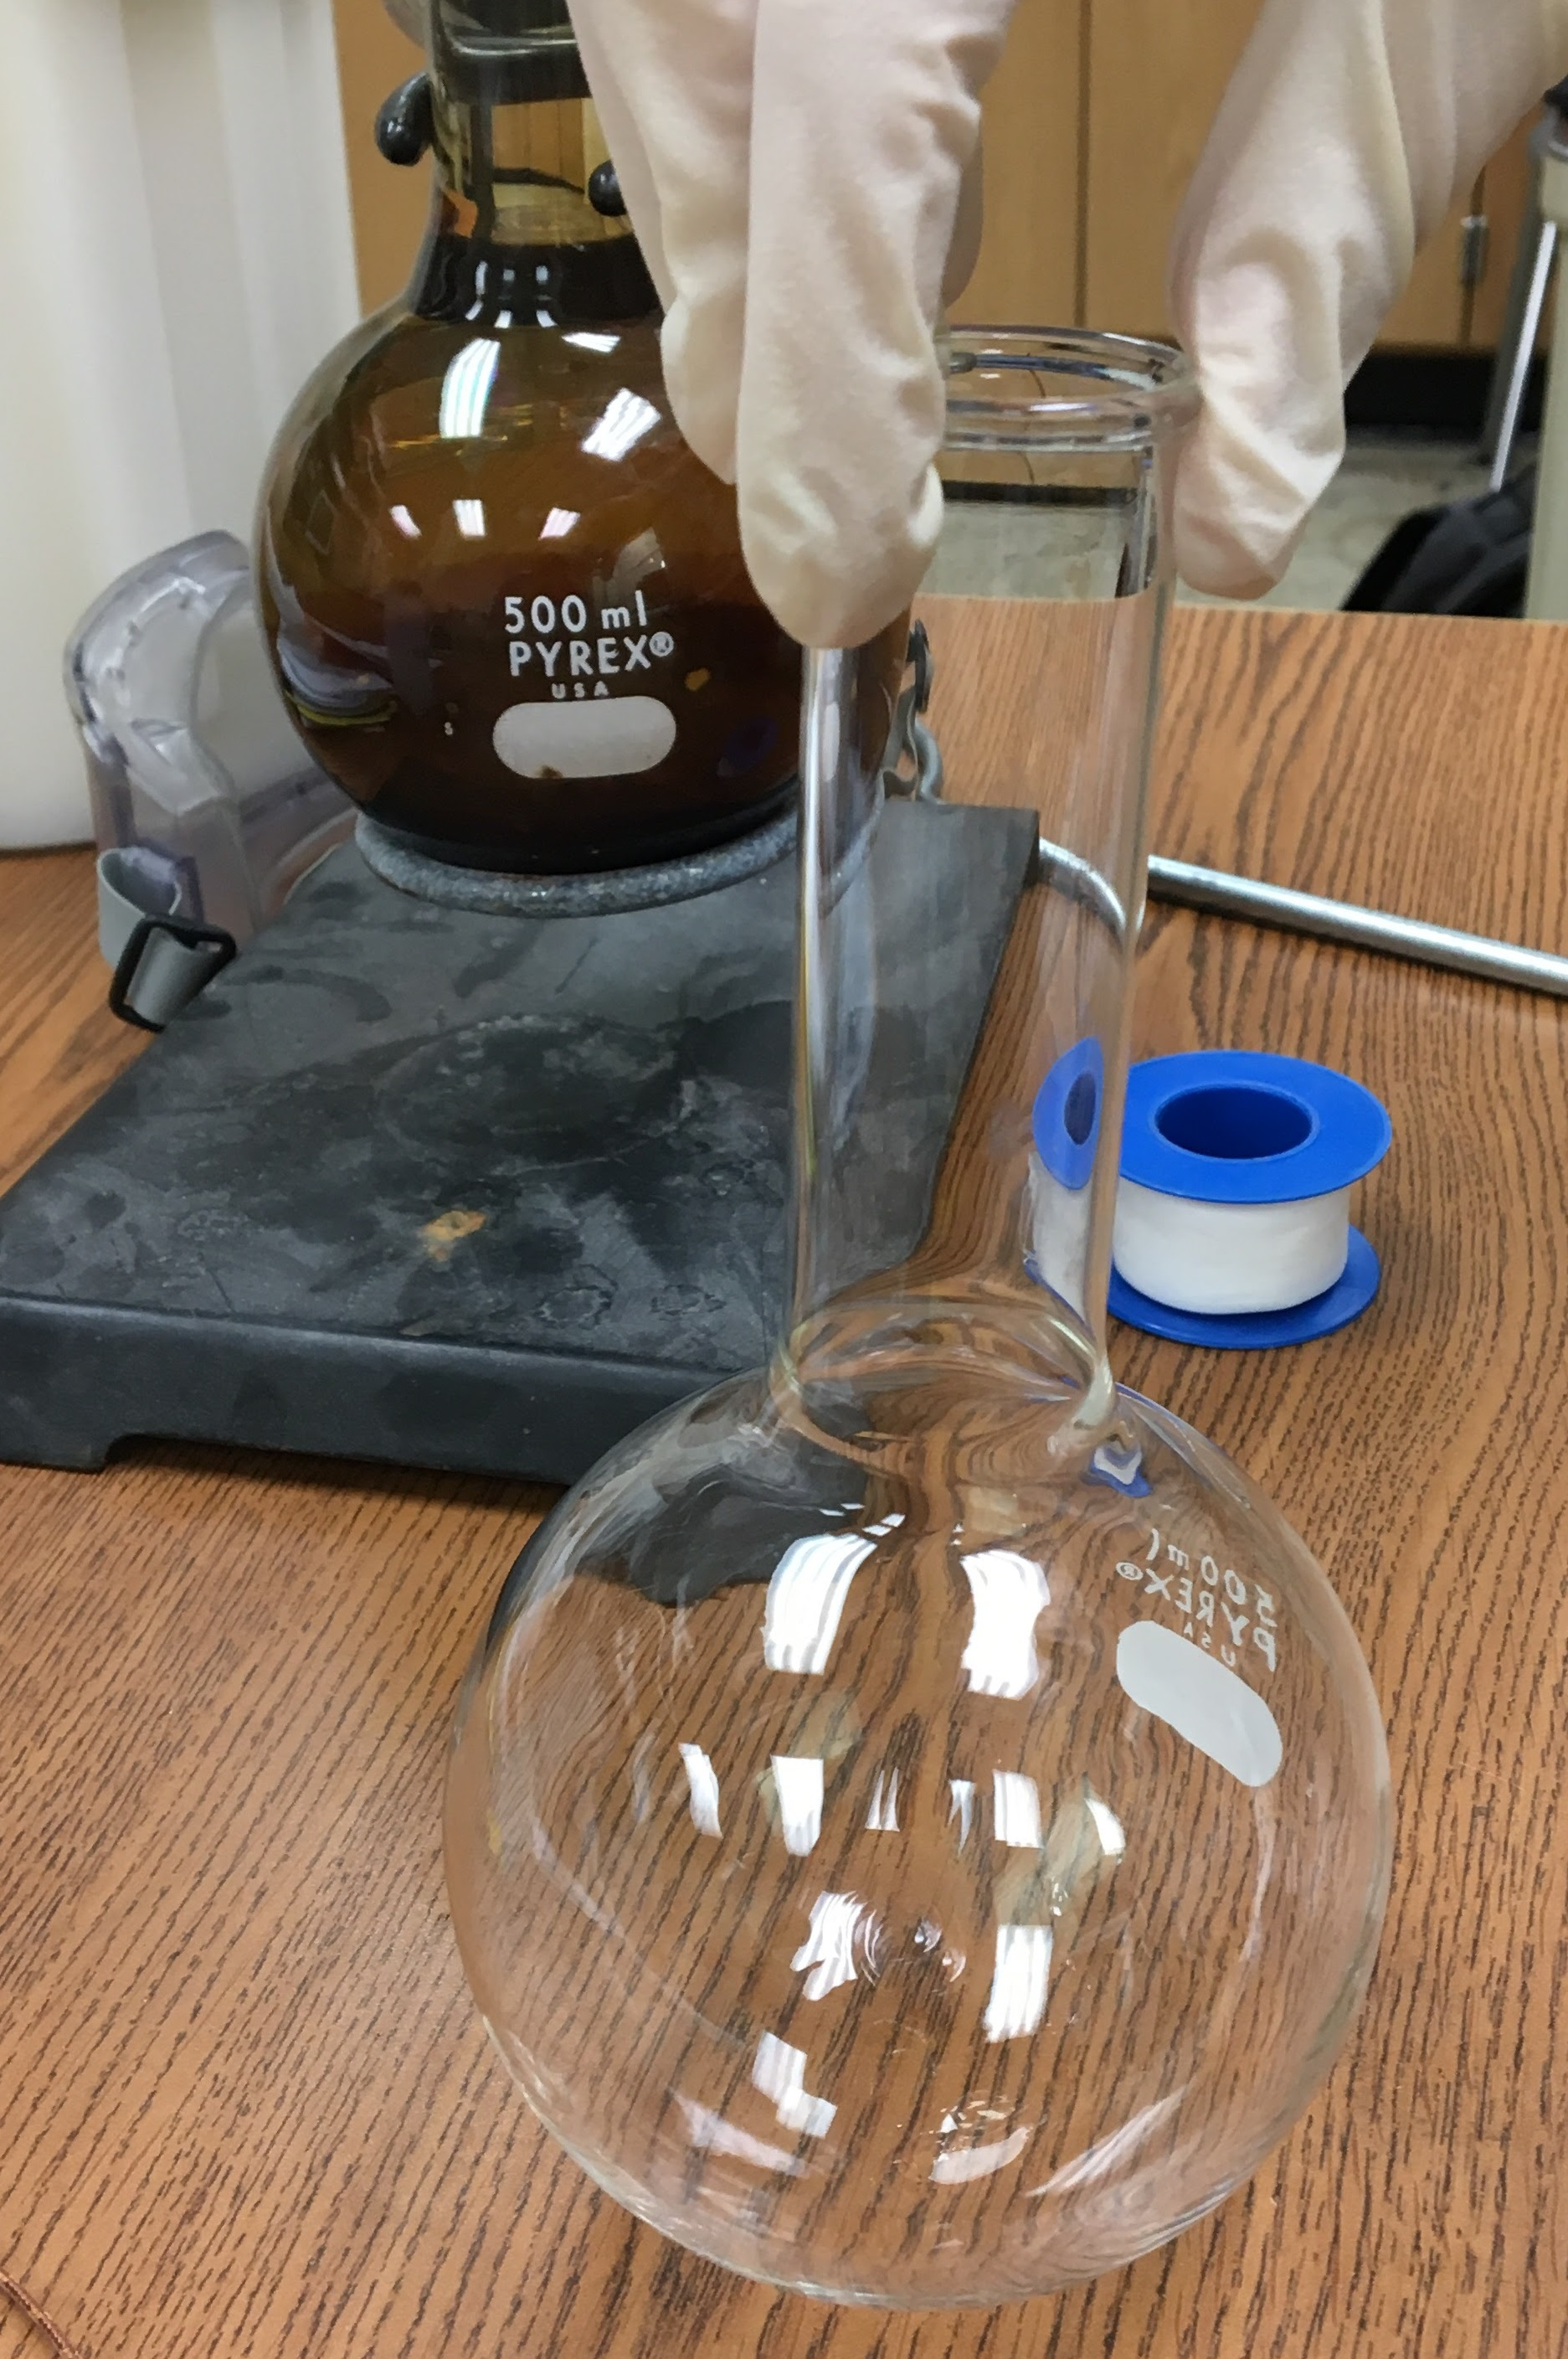
\includegraphics[width=.25\textwidth]{clean_dirty_flask.jpg}
\caption{A clean flask (dirty flask in the background)}
\label{fig:clean_dirty}
\end{figure}  

\newpage 
    \subsection{Furnace}
    \begin{itemize}
    \item The furnace, shown in Figure \ref{fig:furnace_pic}, is an encased 
        stack of ceramic insulation with cavities 
        cut out to allow space for the heating elements and the test flask
        (see Figure \ref{fig:in_furnace} for an internal diagram of the 
        furnace). The furnace is controlled with measurments taken at the 
        insulated furnace wall. This design causes the furnace to have
        large temperature gradients while in operation. As a result, the 
        setpoint temperature and the flask temperature will almost always 
        differ significantly (as much as 25 K in some cases). Therefore, 
        setpoints must be chosen between approximately 10 - 20 K above the 
        desired temperature to reach that temperature inside the flask.
        \textbf{The reported AIT must be taken from the internal flask 
        temperature (Thermocouple 4) and NOT the control thermocouple inside
        the furnace}
    
    \begin{figure}[H]
    \centering
    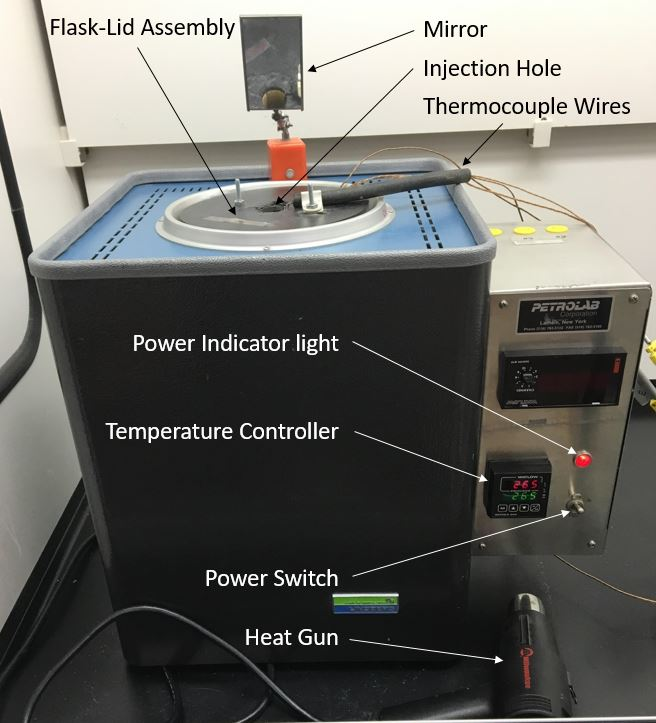
\includegraphics[width=.45\textwidth]{Furnace_pic_diagram.jpg}
    \caption{AIT Furnace}
    \label{fig:furnace_pic}
    \end{figure}
    
    \item When powered on initially, the furnace may take up to 2 hours or more  
        to reach a desired temperature and thermally eqilibrate
    \item Any time a desired temperature is reached, allow at least 30 
        minutes for thorough thermal equilibration in the flask; allow extra 
        time during initial start up

    \item Furnace Operation (See Figure \ref{fig:furnace_pic}):
        \begin{itemize}
        \item Plug in the 220 V extension cord in the corresponding outlet on 
        the wall opposite the hood (adjacent to the DSC computer)
        \item Plug in the furnace to the 220 V extension cord
        \item Power on the furnace with the power switch and use the temperature
            controller to choose a setpoint temperature
        \item To change the set point, press the up or down arrows until 
            the desired temperature is reached
        \item The lower (green) display is the setpoint and the upper 
            (red) display is the control thermocouple temperature
        \item When shutting down, turn off the power switch, unplug the 
            furnace and unplug the 220 V extension cord from the opposite wall
        \end{itemize}
    \end{itemize}

        
    \subsection{Camera and Tablet} \label{sec:cam_tab}
    \begin{itemize}
    \item Prior to using the experimental setup, all researchers must become 
        familiar with basic use and operation of the 
        GoPro\textsuperscript{\textcopyright} HERO4
        Session\textsuperscript{TM} camera and the Samsung Galaxy Tab A Tablet. 
        
        More detailed instructions on how to do basic tasks may be found at the 
        following URLs:
        \begin{itemize}
        \item \texttt{https://shop.gopro.com/softwareandapp}
        \item \texttt{https://gopro.com/help/articles/Block/How-to-Pair-the-Camera-with-the-GoPro-App\#HERO4 Session}
        \item \texttt{https://gopro.com/help/articles/Block/Getting-Started-with-the-GoPro-App}
        \item \texttt{http://www.samsung.com/us/support/owners/product/galaxy-tab-a-8-0-wi-fi}
        \end{itemize}
    
    
\begin{figure}[H]
\centering
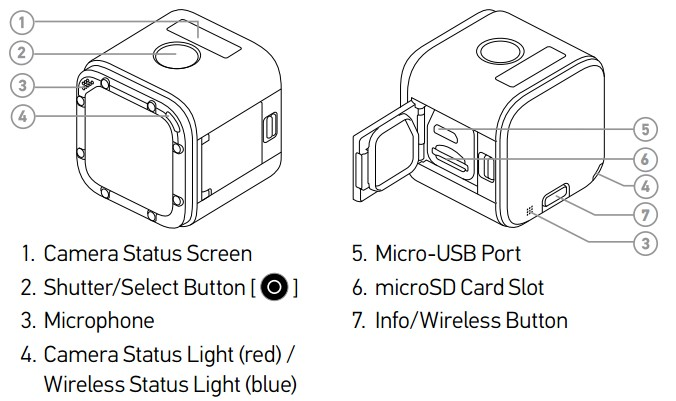
\includegraphics[width=.6\textwidth]{Camera_diagram.jpg}
\caption{GoPro\textsuperscript{\textcopyright} HERO4
        Session\textsuperscript{TM} Camera Parts}
\label{fig:cam_diag}
\end{figure}

\begin{figure}[H]
\centering
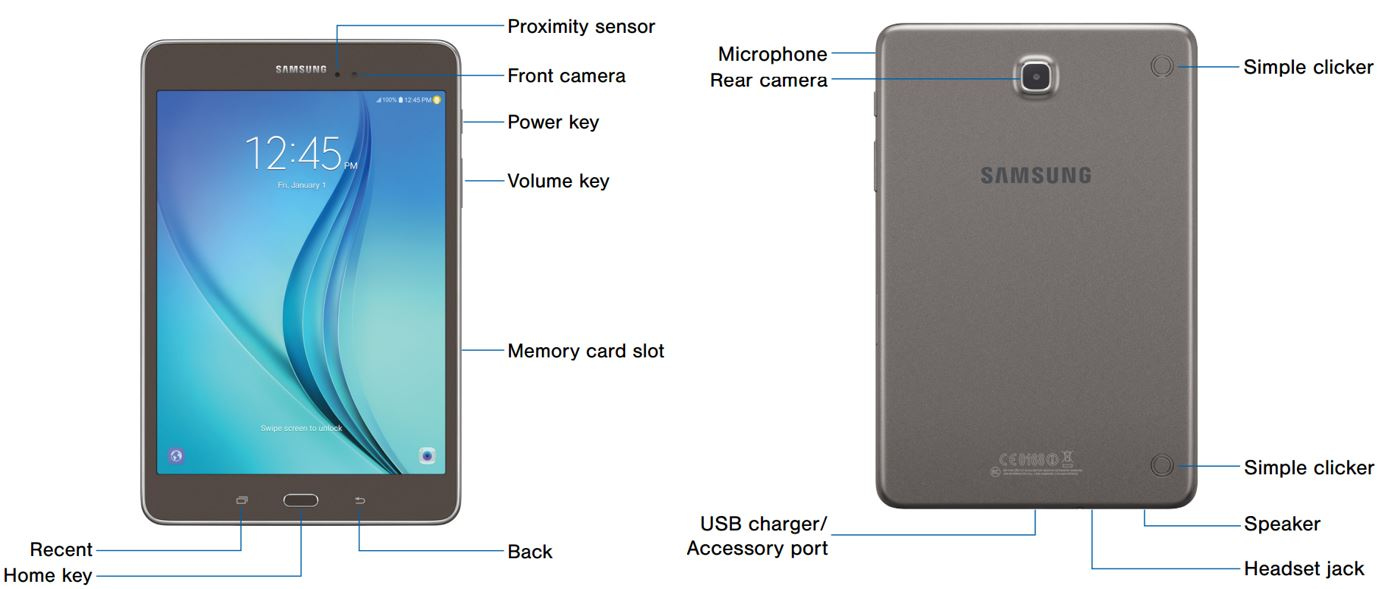
\includegraphics[width=1\textwidth]{tablet.jpg}
\caption{Samsung Galaxy Tab A}
\label{fig:tablet}
\end{figure}
    
    \item Refer to Figures \ref{fig:cam_diag} and \ref{fig:tablet} for camera 
        and tablet setup
    \item Connecting to the camera:
        \begin{itemize}
        \item Press the "info/wireless" button on the back of the camera until 
            you see "APP" on the camera status screen
        \item Press the "shutter/select" button to confirm your selection
            \begin{itemize}
            \item The "wireless status" (blue) light will begin flashing. This 
                indicates the camera is broadcasting a Wi-Fi signal 
            \end{itemize}
        \item Power on the tablet by holding down the power key until you see 
            splash screen indicating the tablet is booting up
        \item Once the tablet has booted, swipe to get to the home screen and 
            select the "Settings" app
        \item Select the Wi-Fi settings at the top of the list on the left side 
            of the screen
        \item Select the Wi-Fi network labeled "ait\_cam\_2016" then select 
            "connect" on the message box that pops up (FYI: the wifi password is
            "hotflame16")
        \item Once the tablet has connected to the Wi-Fi, return to the home 
            screen by pressing the home key
        \item Open the GoPro Capture App (app is labeled "Capture" on the home 
            screen) % CONTINUE HERE!
        \item Select the connect box on the top left corner of the screen
        \item Press the camera icon in the center of the screen
            \begin{itemize}
            \item The camera will make a beeping noise and the camera view will 
                open on the tablet
            \end{itemize}
        \end{itemize}
    
    \item Camera operation:
        \begin{itemize}
        \item All operations may be done remotely on the tablet via Wi-Fi or 
            directly with the "info/wireless" and "shutter/select" buttons on 
            the camera. For experimental purposes, only basic operations
            will be covered. For more detail on camera 
            operation please see the URLs above
        \item In the camera's off or normal modes the "shutter/select" button 
            toggles recording or standby; the camera will automatically shut off
            after a few seconds on standby
        \item If the camera is remotly controlled, the on screen red button 
            toggles recording or standby
        \item During recording, the camera will not allow viewing via the 
            tablet. This is due to the high framerate of our experiments
        \item Captured video may be reviewed and managed remotely with the grid
            button on the bottom left corner of the screen
        \item The camera may be powered on and off remotely with the power  
            button on the top right corner of the screen. The camera should be 
            powered off between experiments or when not in use
        \end{itemize}
    
    \item Shutdown:
        \begin{itemize}
        \item To shutdown the camera:
            \begin{itemize}
            \item Press the "info/wireless" button 
                until the camera status screen reads "Turn Wi-Fi Off"
            \item Press the "shutter/select" button to confirm your selection
                \begin{itemize}
                \item The "wireless status" (blue) light will stop flashing
                \end{itemize}
            
            \item Press the "info/wireless" button until the camera status 
                screen reads "Exit"
            \item Press the "shutter/select" button to confirm your selection
                \begin{itemize}
                \item The camera will shutdown 
                \end{itemize}
            
            \end{itemize}
        
        \item To shutdown the tablet:
            \begin{itemize}
            \item Press the "Recent" button to bring up all opened programs and 
                close all programs by swiping on them or pressing the 'X' in the
                top right corner
            \item Press and hold the Power key until the option to power of 
                pops up then press power off
                \begin{itemize}
                \item The tablet will shutdown
                \end{itemize}
           
            \end{itemize}
        
        \end{itemize}
    
    \item Batteries:
        \begin{itemize}
        \item Recharging power supplies and usb cables are availible for both
            the tablet and camera
        \item Both the camera and the tablet may be charged while in use
        \item Do NOT charge tablet with the computer as it does not deliver 
            enough current for effective charging
        \item Batteries should be allowed to discharge to between 10 - 20\%
            before recharging
        \item Batteries should always be recharged to 100\% capacity before 
            unplugging
        \item Do not overcharge any battery. Do not leave any battery 
            charging overnight
        \end{itemize}
        
    \end{itemize}
    
    %\subsection{TA-DA}
    
\newpage % NEW SECTION OF DOCUMENT

\section{Measurement and Data Collection}
This section enumerates the procedure for measuring AIT. Researchers 
should follow these procedures every day and for every experiment performed to 
ensure consistent results. The first priority should always be safety. 
Therefore, if any step of this process is found to be unsafe or pose an 
unacceptable risk it should be changed. Furthermore, changes should be made if 
any step of the process violates the ASTM E659 Method to conform to the 
requirements of the method.
    
    \subsection{Startup}
    \begin{enumerate}
    \item Plug in the 220 V extension cord in the corresponding outlet on 
        the wall opposite the hood (adjacent to the DSC computer)
    \item Plug in the furnace to the 220 V extension cord
    \item Power on furnace and set furnace temperature between 20 - 30 degrees 
        above your initial target flask temperature 
    \item Reduce the set point temperature when the internal flask temperature 
        exceeds your initial target temperature by 5 - 10 degrees 
        \begin{itemize}
        \item Wait a minimum of 90 minutes before changing the temperature
        \item When powered on initially, the furnace may take up to 2 hours or   
            more to reach a desired temperature and thermally eqilibrate
        \end{itemize}
    
    \item Start up computer and log on
        \begin{itemize}
        \item Use your CAEDM account to log in
            \begin{itemize}
            \item You should be able to access all the needed tools and 
                programs from your account
            \item If you cannot access a program or file from your account, let 
                me know and I will give you administrator access as needed
            \end{itemize}
        
        \item You may need to specify the domain you are logging into. If that 
            is the case enter your CAEDM credentials in as follows:
            \begin{itemize}
            \item Username: CAEDM\_AD\textbackslash
            \textit{your\_caedm\_username}
            \item Password: \textit{your\_caedm\_password}
            \end{itemize}
        
        %\item Using the administrator account:
        %    \begin{itemize}
        %    \item Username: CHEME-R-2014-25\textbackslash AIT\_LAB
        %    \item Password: Explosionsinthesky16 (Explosions in the sky 16)
        %    \end{itemize}
        
        \end{itemize}
    
    \item Ensure a compatible SD card is inserted securely into the TA-DA 
        datalogger
    \item Ensure the thermocouples are connected to the TA-DA

    \item Connect the TA-DA to the lab computer via the USB cable mounted 
        under the edge of the hood
    
    \item Open the TA-DA user interface program 
            \begin{itemize}
            \item Path: \textit{C:\textbackslash Users\textbackslash  
                Public\textbackslash Documents\textbackslash AIT\textbackslash 
                tools\textbackslash TADA\_UI.py}
            \item You may wish to make a shortcut to this location and put it on 
                your CAEDM desktop.
            \item Upon opening the program, a yellow LED in the TA-DA should 
                begin flashing (See Figure \ref{fig:tada_leds})
            \end{itemize}

\begin{figure}[H]
\centering
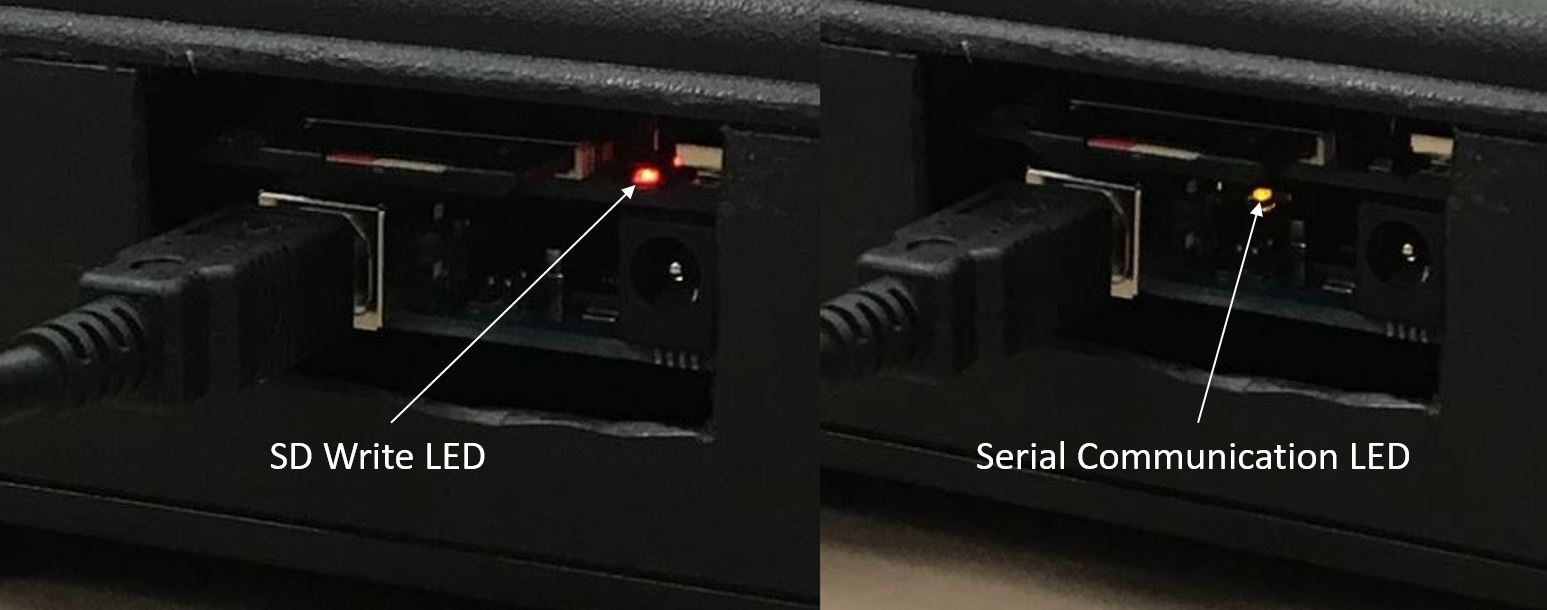
\includegraphics[width=.75\textwidth]{led_red_yellow.jpg}
\caption{Control LEDs inside the TA-DA}
\label{fig:tada_leds}
\end{figure}
    
    \item Press the "Sync Time" button on the bottom left corner of the TADA\_UI
        window to syncronize the arduino clock to the computer time
        \begin{itemize}
        \item This must be done at least once every work day
        \end{itemize}
        
    \item Use the TADA\_UI program to track the internal temperature of the 
        flask as it heats up initially
    \item Prepare the tablet and the camera
        \begin{itemize}
        \item Power on the tablet and connect it to the camera's Wi-Fi (See 
            Section \ref{sec:cam_tab} on how to do this)
        \item Open the capture app to view the camera's view finder
        \item Mount the camera on the tripod in the hood using the quick-release
            plastic camera mount on top of the tripod
        \item Using the camera's view finder on the tablet, adjust the
            position of the camera, tripod and mirror on the furnace to 
            align the camera's view directly down the center of the flask
            \begin{itemize}
            \item The camera should be positioned approximately level with the 
                 top of the furnace looking slightly upward into the mirror
            \item For the best view, the camera should be as close to the 
                furnace as the tripod will allow and pointed directly into 
                the mirror
            \end{itemize}
        
        \item Gently tighten the knobs on the tripod to fix the camera in place
        \item Close the hood sash
        \end{itemize}
    
    \item Place a piece of cardboard or other opaque sheet on the right side 
        of the hood against the outer sash and tuck it into the edges of the 
        space between the sash and the hood wall so that it blocks light from 
        entering the hood
    \item Once the target temperature is reached, allow 30 minutes for thermal 
        equilibration then begin experiments
    \end{enumerate}
    
    \subsection{Experimental}
This section outlines the steps for experimental runs. Each experiment should be
performed following these steps exactly (insofar as that is possible). Doing so
will ensure consistent results with the lowest uncertainty possible.
    \begin{enumerate}
    \item Measure the absolute pressure in the lab with the mercury barometer 
        mounted on the west wall by the sink and write down the pressure
        in the lab notebook
    \item Measure the relative humidity and ambient temperature in the hood  
        with the hygrometer and write down those values in the lab notebook
        \begin{itemize}
        \item Remove the cap from the hygrometer probe and set the probe inside 
            the hood away from the furnace
        \item Press the "ON/OFF" button on the hygrometer to turn the unit on
        \item Press "MODE" until the unit displays the relative humidity
        \item Wait 1 minute to allow the unit to equilibrate
        \item Write down the value for the relative humidity in the lab notebook
        \item Press "MODE" again until the temperature is displayed
        \item Write down the value for the ambient temperature in the lab 
            notebook
        \item Turn off the unit by pressing the "ON/OFF" button, remove the 
            probe from the hood and put the probe cap back on and store the unit
            in its case
        \item For more information on the proper use of the hygrometer, refer to 
            the instructions in the hygrometer case
        \item Do \textbf{NOT} leave the probe sitting in the hood for an 
            extended period of time without its cap on. The hygrometer probe is 
            sensitive to dust and debris and can be easily damaged if left in 
            the hood
        \end{itemize}
        
    \item In the TADA\_UI program, press the "Choose Target File" button and 
        choose where to save your file
        \begin{itemize}
        \item Save all temperature data files in comma separated values (.csv) 
            format
        \item Path: \textit{C:\textbackslash Users\textbackslash 
            Public\textbackslash Documents\textbackslash AIT\textbackslash 
            data\textbackslash compound\_name\textbackslash filename.csv}
        \item File naming convention: 
            \begin{itemize}
            \item Filenames will be organized by the following values in order 
                separated by underscores ("\_")
                    \begin{itemize}
                    \item Compound name
                    \item Phase of the compound ('g' for gases, 'l' for liquids,
                        's' for solids)
                    \item Date of experiment with the format "YYMMDD"
                    \item Time of day that data collection began for that run
                        using a 24 hour clock format "hhmm"
                    \item Sample size in microliters (for liquids) or milligrams
                        (for solids and gases)
                    \item Test temperature in degrees Celsius (rounded to the 
                        nearest integer)
                    \end{itemize}
                    
            \item For example: The filename of an AIT experiment where 100 
                microliters of liquid hexane were tested at 450 \degree C on 
                March 19, 2013 at 4:25 pm would be: \newline
                "hexane\_l\_130319\_1625\_100\_450\_.csv"
            \end{itemize}    
        \item This action will reset the TA-DA for the next measurement        
        \end{itemize}
    
    \item \textbf{Safety: Ensure you are using proper PPE and have minimized 
        hazards in the lab environment before continuing}
            
            \begin{itemize}
            \item Ensure your workspace, the area around the computer and 
                both hoods are free of clutter, tripping hazards or any object 
                which could present a hazard to you or anyone else in the lab
            \item Appropriate PPE (e.g. nitrile gloves and splash goggles) are 
                required when handling chemicals
            \item Refer to the SDS for the chemical you are working 
                with when determining appropriate PPE
                \begin{itemize}
                \item NOTE: Some SDS's will recommend using a face shield in 
                    addition to splash goggles when handing their respective 
                    chemicals. In our lab we will use ventilation hoods which, 
                    when used properly, serve as better protection than face 
                    shields. Therefore, any time an SDS recommends using a 
                    face shield you may safely ignore that recommendation 
                    provided you are using the hood properly by positioning the 
                    sash between your face and the work being performed in 
                    the hood.
                \end{itemize}
                
            \item Unless an SDS states otherwise, lab coats are recommended but 
                not required when handling chemicals
            \item All chemical handling (except for injection into the furnace) 
                should be done in the left hood to avoid a potential fire hazard 
            \end{itemize}
    

    \item Measure out sample
        \begin{itemize}
        \item Liquids
            \begin{itemize}
            \item Draw sample amount into a right-angle syringe            
            \end{itemize}
        
        \item Solids
            \begin{itemize}
            \item Measure out sample in a weigh boat on the lab scale
            \item Use a powder funnel to inject the sample into the furnace
            \item Keep the funnel as close to vertical as possible during 
                injection to minimize the amount of compound that does not enter
                the flask
            \end{itemize}
            
        \item Gases
            \begin{itemize}
            \item Draw sample amount into a right-angle syringe           
            \end{itemize}
            
        \end{itemize}
    
    \item Set the measured sample aside in the left hood
    \item Remove any glove from your LEFT hand and use your left hand for 
        touching any non-hazardous surfaces
    \item Ensure the lab is sufficiently dark to see any flame from the mirror
        on top of the furnace
        \begin{itemize}
        \item Use the lights in the hoods for preparation before your run
        \end{itemize}
    
    \item With your LEFT hand, press the Enter key to 
        initiate data collection (a red LED in the TA-DA should begin blinking)
        \begin{itemize}
        \item The TA-DA UI will keep track of the elapsed time since data 
            collection began at the bottom of the window. This may be used
            to time the experiment
        \end{itemize}
    \item With your LEFT hand, press the red button on the tablet screen to 
        start recording
    \item With your LEFT hand, open the sash horizontally just enough that your
        RIGHT hand can inject the sample
    \item With your RIGHT (gloved) hand, retrieve your sample and center the 
        end of the syringe or funnel in the hole at the top of the furnace for 
        injection, ensuring that the sample will go straight down and not hit 
        the sides of the flask
    \item Simultaneously turn off the light in the hood (with your LEFT hand) 
        and introduce your sample (with your RIGHT hand) (the light turning off 
        indicates to the camera that the sample has been injected)
        \begin{itemize}
        \item Immediately withdraw the syringe or funnel, close the sash (with 
            your LEFT hand) and place the syringe in the adjacent hood
        \item Begin the 10 minute timer
        \item \textbf{NOTE ON EXPERIMENTS WITH SOLIDS:} When experimenting with 
            solids, it is difficult for one person to simultaneously introduce a 
            sample, hold the funnel in place and turn off the light. Therefore 
            for solid experiments, have a second person there to turn off the 
            light as the sample is injected. If a second person is present, 
            he/she must also wear appropriate PPE for the experiment. (i.e. The
            second person must wear PPE corresponding to the compound SDS but 
            must NOT be wearing gloves when switching off the light.)

            If no one is available to do this, the light may be turned off 
            quickly after introducing the sample and removing the funnel. In 
            this case, the camera should be able to view the sample entering the
            flask and have an accurate time of injection.
        \end{itemize}    
            
    \item Watch the mirror above the furnace for any flame/glow or the TA-DA UI
        for a large temperature spike for 10 minutes
        \begin{itemize}
        \item If a flame, glow or spike is observed, stop the camera after the 
            flame disappears and then allow enough time for the temperature to 
            return to a steady state before terminating temperature data 
            collection
                \begin{itemize}
                \item If the flame is bright yellow/orange, this is considered a 
                    hot-flame autoignition
                \item If the flame is faint and blueish, this is considered a 
                    cool-flame autoignition
                \end{itemize}
        
        \item The experiment ends when one of the following criteria is met:
            \begin{itemize} 
            \item An ignition event is observed (i.e. a temperature spike or 
                seeing a flame) and the temperature returns to steady state
            \item 10 minutes pass with no ignition event observed
            \end{itemize}
        \item If the UI is used to keep track of time and no flame is observed, 
            continue collecting temperature data until 700 seconds have passed 
            to ensure the full 10 minutes of data have been captured
        \end{itemize}
    
    \item Record pertinent data and observations in the lab book and the 
        TA-DA UI
        \begin{itemize}
        \item The following data must be present on the same row, in the 
            following order:
            \begin{itemize}
            \item Time of day that data collection began for that run
            \item Compound name 
            \item The lot number and/or sample number of the 
                container (This only needs to be recorded in the lab book  and 
                only once for every compound container)
            \item Phase of the compound upon injection ('g' for gases, 'l' for 
                liquids, 's' for solids)
            \item Sample size in microliters (for liquids) or milligrams
                (for solids and gases)
            \item Set-point temperature of the furnace
            \item Test temperature in degrees Celsius (rounded to the 
                nearest integer)
                \begin{itemize}
                \item This should be the internal flask temperature 
                    (Thermocouple 4) prior to injection
                \end{itemize}
            \item Indicate whether an ignition event was observed (i.e. Did you 
                or the camera see a flame?)
            \item Indicate whether a hot flame or cold flame was observed (if 
                applicable)
            \item Indicate if any sound was heard upon ignition (if applicable)
            \item The barometric pressure at the time of the experiment 
                (in mmHg)
            \item The relative humidity (\%) and the ambient air temperature
                in the hood
            \end{itemize}

        \item If any item is not applicable write down N/A in its place
        \item If any item is unknown, leave a blank until it can be determined
        \item Optionally, leave any pertinent comments about the experiment
            next to or directly under this row of data
        \item Record the same data in the corresponding fields in the TA-DA UI
            \textbf{before} terminating temperature data collection
        \end{itemize}
        
    \item After the experiment ends, terminate data collection
        \begin{itemize}
        \item Press the Enter key  again to stop data 
            collection (the red light on the TA-DA should stop blinking)
        \item Press the red button on the tablet screen to stop recording
        \item Turn the lights back on
        \item Video recording may be stopped as soon as a flame or glow
            disappears
        \end{itemize}

    \item Prepare for the next measurement
        \begin{itemize}
        \item Set furnace to next temperature
            \begin{itemize}
            \item When changing temperature, always approach your target
                temperature from 5 - 10 degrees Celsius above and then 
                descending slowly to your target temperature
            \item This practice is intended to control for hysteresis effects
                (See Section \ref{sec:hyst})
            \end{itemize}
        \item Clean out the flask between measurements by blowing hot air into 
            the flask for 5 minutes using the heat gun
            \begin{itemize}
            \item The heat gun should \textbf{only} be plugged in to the outlet 
                when in  use
            \end{itemize}

        \item Extract, save and appropriately rename the video data between 
            experiments
        \item Wait a minimum of 30 minutes to reach the new temperature and 
            allow the furnace and flask to thermally equilibrate
        \end{itemize}
    
    \item Start this procedure over from step 1 (measure the pressure)
    \end{enumerate}
    
    \subsection{Shutdown}
    \begin{itemize}
    \item The following should be done before leaving the lab at the end of 
        every work day or anytime the setup is not in use:
        \begin{itemize}
        \item Power off the furnace
        \item Unplug the furnace from the 220 V extension cord
        \item Unplug the 220 V extension cord from the wall opposite the hood
        \item Unplug TA-DA from the computer 
        \item Tuck the end of the USB cord into the mounted section under the 
            edge of the hood so it does not present a tripping hazard
        \item Extract all data to the computer and appropriately rename them
        \item Shut down and unplug the tablet and the camera
        \item Remove the cardboard from the hood and stow it between the hood 
            and the toolbox
        \item Remove the camera from the tripod using the plastic quick-release 
            lever and store the camera next to the lab computer
        \item Put all chemicals and syringes away in their proper places
        \item Remove any organic solid residue from all working surfaces 
            (See Section \ref{sec:spill_solid})
        \item Close all programs and shutdown the computer
        \end{itemize}
    
    \item A hot furnace may be left in the hood without waiting for it to cool
    \item Do not rinse out needles %% add policy for needles !!!!!!!
    \item Under normal use, disposable gloves may be thrown into the normal 
        trash receptacle instead of solid chemical waste
    \end{itemize}
    
\section{Data Extraction} 
During experiments data are being recorded on the lab computer, the datalogger 
and the camera. Both the camera and the datalogger on the TA-DA have SD cards 
with a 32 GB storage capacity that allows multiple runs to be recorded without 
extraction. The following policies are in place to ensure ease of use, 
efficiency and avoid common mistakes.
    \begin{itemize} 
    \item For the AIT setup, do not exceed 10 runs without extracting 
        temperature data to the computer and deleting the data from the SD  
        cards.
    \item All data should be extracted at least \textit{daily}
    \item Video data should be extracted and properly renamed as often as  
        possible (i.e. between every run or every other run) to ensure the 
        correct filenames are assigned to their corresponding video files
    
    \item File naming convention: 
        \begin{itemize}
        \item Filenames will be organized by the following values in order 
            separated by underscores ("\_")
                \begin{itemize}
                \item Compound name
                \item Phase of the compound ('g' for gases, 'l' for liquids,
                    's' for solids)
                \item Date of experiment with the format "YYMMDD"
                \item Time of day that data collection began for that run
                    using a 24 hour clock format "hhmm"
                \item Sample size in microliters (for liquids) or milligrams
                    (for solids and gases)
                \item Test temperature in degrees Celsius (rounded to the 
                    nearest integer)
                \end{itemize}
                
        \item For example: The filename for temperatures from an AIT experiment  
            where 100 microliters of liquid hexane were tested at 450
             \degree C on March 19, 2013 at 4:25 pm would be: \newline 
            "hexane\_l\_130319\_1625\_100\_450.csv"
        \end{itemize}

    \item Video and datalogger data must be processed (i.e. parsed, edited, 
        timestamped etc.) before being organized and therefore will be saved to 
        a different path initially

    \item After processing, all data should be organized according to the 
        following path convention:
        \begin{itemize}
        \item Path: \textit{C:\textbackslash Users\textbackslash 
            Public\textbackslash Documents\textbackslash AIT\textbackslash 
            data\textbackslash compound\_name\textbackslash filename.ext}
        \item All data, including videos, from the same run should have the same
            filename and path but different extensions except data from the 
            datalogger
        \item The datalogger filename convention should also have '\_dlog' at 
            the end of the name to distinguish it from the UI generated file 
            (e.g. "hexane\_l\_130319\_1625\_100\_450\_dlog.csv")
        \item When processing is finished all runs should have the following 
            4 files with the same name preceding them
            \begin{itemize}
            \item A .xlsx file (for temperature data w/ graphs and analysis)
            \item A .csv file (UI generated)
            \item A \_dlog.csv file (datalogger)
            \item A .avi/.mp4 file (video)
            \end{itemize}
        \end{itemize}

    \item The camera may be plugged in via USB and video extracted with
        GoPro\textsuperscript{\textcopyright} Quik software
        \begin{itemize}
        \item Connect the camera to the computer via a micro USB cable (See 
            Figure \ref{fig:cam_diag})
        \item Press the "info/wireless" button on the camera to connect the 
            camera to the computer
        \item Quik should be configured to open automatically extract video and 
            erase the microSD card when the camera connects to the computer
        \item Video files should be extracted to the DIPPR legacy server and 
            organized by date:
            \begin{itemize}
            \item Path: \textit{\textbackslash \textbackslash 
               dipprlegacy.et.byu.edu\textbackslash aitra\textbackslash 
               video\_import}
            \item Username: dipprleg\textbackslash aitra
            \item Password: hotflame16
            \end{itemize}
        \item If Quik is not configured to do this refer to the Quik manual for
            how to configure this (or ask me and I will configure it)
            \begin{itemize}
            \item \textit{C:\textbackslash Users\textbackslash 
            Public\textbackslash Documents\textbackslash AIT\textbackslash 
            docs\textbackslash GoPro\_App\_for\_Desktop\_User\_Manual.pdf}
            \end{itemize}
        \item Once extracted to the DIPPR legacy server, video data may be 
            timestamped and converted to .avi format on the server (See 
            Section \ref{sec:data_pa})
        \end{itemize}
        
    \item To extract data from the datalogger
        \begin{itemize}
        \item Unplug the TA-DA from the computer
        \item Pull out the SD card from the datalogger and use the USB SD card 
            adapter to copy the"DATALOG.CSV" file into the "raw\_data" path and 
            rename it to the original filename with the date 
            tagged on in "YYMMMDD" format (e.g. "DATALOG\_130319.CSV")
            \begin{itemize}
            \item Path: \textit{C:\textbackslash Users\textbackslash 
            Public\textbackslash Documents\textbackslash AIT\textbackslash 
            data\textbackslash raw\_data}
            \end{itemize}
        \item Open the "DATALOG.CSV" file on the SD card, erase all data from
            it and save it, making sure to not change its name, extension or 
            file path
        \item Close all windows with the USB SD card adapter open (i.e. Excel 
            files, Windows Explorer etc.)
        \item Pull out the SD card without ejecting the unit from the computer
        \end{itemize}
    
    \item Ensure all files from the camera and datalogger are deleted after they
        have been properly saved in the data folder 
            
    \end{itemize}

\newpage % NEW SECTION OF DOCUMENT 
%\blankpage
\section{Experimental Design}
This section outlines basic principles for finding the AIT of a compound from 
perspective of experimental design.
This section must be read at least once to be authorized to work on AIT. 
However, understanding all the steps in this section is optional to begin 
experimental work. It is expected that researchers will become familiar with and
understand these steps over time after some experience measuring AIT.

The other sections of this SOP concern matters related to saftey and precise, 
consistent measurement and should be followed exactly to ensure the best 
results. This section, however, deals with a much more nuanced view of AIT and
how to find the minimum value. Because of this, the steps and procedures in this
section may be taken as flexible guidelines rather than imperative rules. They
should inform decisions made by researchers rather than perscribe them. With 
this in mind, these are the guidelines for some specifics on how to measure AIT.

The following principles should guide all decisions regarding AIT measurement:
\begin{itemize}
\item \textbf{The autoignition temperature is defined as the minimum temperature 
    at which hot-flame ignition occurs in the absence of an ignition source}
    \begin{itemize}
    \item Hot-flame ignition is defined as seeing a yellow/orange/red part of a 
        flame or glow associated with the ignition event
    \item Cool-flame ignition is defined as seeing an entirely blue flame or 
        glow associated with the ignition event
    \end{itemize}
\item \textbf{The reported AIT must be the internal flask temperature 
    (Thermocouple 4) and NOT the temperature of the furnace}
    \begin{itemize}
    \item The best measure available for AIT in the ASTM method is having the
        AIT be the air temperature prior to injection inside the flask
    \end{itemize}

\item \textbf{The bracket size goal for AIT measurement is $\pm$ 3 \degree C}
    \begin{itemize}
    \item This means that if a hot-flame ignition can be consistently measured  
        at a certain temperature and a cold flame can be consistently measured  
        $< 3$ degrees below it, the hot-flame temperature should be reported as 
        the measured AIT
    \end{itemize}
\end{itemize}
    
    \subsection{Guidelines for Finding AIT} \label{sec:guide}
    \begin{itemize}
    \item A more complete and precise definition of AIT as per ASTM E659: The 
        minimum temperature of a fuel/air mixture at which hot-flame 
        ignition occurs, in the absence of an ignition source, for a system that
        meets the following criteria:
        \begin{itemize}
        \item The fuel/air mixture is contained in a 500 ml borosilicate 
            bulb flask
        \item The bulb flask is open to the atmosphere
        \item The bulb flask is at a uniform temperature
        \item Both the bulb flask and the air inside are at steady state 
            temperatures immediately before the fuel is introduced
        \item The composition of the air in the flask is 20.95\% oxygen with the
            balance being inert gases
        \item The barometric pressure of the system is 1 atmosphere
        \item The fuel to air ratio is optimized to minimize the AIT
        \end{itemize}
    
    \item The experimental setup has been designed to conform to these criteria
        insofar as it is practical to do so. Changes will be made continually
        to the setup to better match these criteria.
    \item To choose temperatures to be tested the following guidelines may be 
        useful:
        \begin{itemize}
        \item If there are any data that indicate where the AIT is, start there
        \item If there are no data for a compound look at the compound's family 
            and interpolate from those data to choose a starting temperature
        \item If there are no data for a compound or its family find a compound 
            with data that most resembles your compound and start at that 
            compound's AIT
        \item Once a starting point is found, begin with a broad strokes 
            approach by jumping up and down by 30 degrees Celsius or more until 
            you bracket the minimum AIT with hot-flame and cold flame ignitions
        \item Shrink that bracket with a bisection method until the bracket is 
            $<$ 3 degrees Celsius
        \end{itemize}
    
    \item Once a minimum AIT is found for a baseline sample size, vary the 
        sample size (See Section \ref{sec:samp_sz}) and repeat the procedure 
        above until you find a minimum AIT with an optimum sample size
    \end{itemize}
    
    \subsection{Furnace/Flask Temperatures} \label{sec:hyst}
    \begin{itemize}
    \item We have observed some hysteresis effects in how we approach the 
        temperature to be tested. We have noticed if we start high and drop down
        to the desired temperature the AIT tends to be lower than if we start 
        low and heat up to the desired temperature.
    \item To control for these effects, we strongly recommend always 
        overshooting higher than the temperature needed and then backing off the
        heat to allow the temperature to fall to the desired value. Doing so
        should control for the hysteresis effects observed.
    \item The flask temperature (Thermocouple 4) should be monitored while 
        temperatures change to check for steady state. From tests on the 
        response curve of the furnace, we have determined that the time constant
        of the system is roughly 10 minutes and the dead time is about 2 minutes 
        which would mean that within 30 - 35 minutes the flask should come close
        to steady state. If the temperature changes less than 3 degrees Celsius 
        over 10 minutes researchers may always consider the system at steady 
        state.
    \end{itemize}
    
    \subsection{Sample Size} \label{sec:samp_sz}
    In Section \ref{sec:guide} the guidelines for finding AIT were covered with 
    respect to temperature. This section lays out guidelines for how to choose 
    a sample size and how to store and inject. Before varying sample size, 
    researchers should generally find an AIT for the current sample size

    \begin{itemize}
    \item Liquids
        \begin{itemize}
        \item Draw sample amount into a right-angle syringe
        \item Sample size:
            \begin{itemize}
            \item Initially use a sample size of 100 microliters
            \item Once AIT is measured for 100 microliters, go to 150 
                microliters
            \item If the AIT decreases for 150 microliters, go to 200/250 
                microliters
            \item If the AIT increases for 150 microliters, go to 50 
                microliters
            \end{itemize}
        
        \end{itemize}
            

    \item Solids
        \begin{itemize}
        \item Measure out sample in a weigh boat on the lab scale
        \item Use a powder funnel to inject the sample into the furnace keeping
            the funnel vertical to minimize the amount of compound not entering 
            the furnace
        \item Sample size:
            \begin{itemize}
            \item Initially use a sample size of 100 milligrams
            \item Once AIT is measured for 100 milligrams, go to 150 
                milligrams
            \item If the AIT decreases for 150 milligrams, go to 200/250 
                milligrams
            \item If the AIT increases for 150 milligrams, go to 50 
                milligrams
            \end{itemize}
        
        \end{itemize}
        
    \item Gases
        \begin{itemize}
        \item Draw sample amount into a right-angle syringe
        \item Sample size:
            \begin{itemize}
            \item Initially use a sample size of 100 milligrams
            \item Once AIT is measured for 100 milligrams, go to 150 
                miligrams
            \item If the AIT decreases for 150 miligrams, go to 200/250 
                miligrams
            \item If the AIT increases for 150 miligrams, go to 50
                miligrams
            \end{itemize}
        
        \end{itemize}
    
    \end{itemize}

    
    \subsection{Flame and Glow}
    The following are guidelines for flame observation:
    \begin{itemize}
    \item If the flame is at least partly bright yellow, orange or red, this is 
        the hot-flame autoignition and the temperature should be 
        decreased for the next test
    \item If the flame is faint and blueish, this is the cool-flame 
        autoignition and the temperature should be increased for 
        the next test
    \item If no flame or glow if observed by the 10 minute mark, 
        increase the temperature for the next measurement
    \end{itemize}


\section{Data Processing and Analysis (Section is in ALPHA)} \label{sec:data_pa}
\textbf{NOTE: This section is in ALPHA stage of development and does not outline any 
procedures that are necessary for safety in the lab. Therefore, until this
section is taken out of ALPHA stage the material in this section is optional and
not considered part of the SOP. This means that you may skip this and any 
sections in ALPHA stage when reading the entirety of the SOP as required for lab
work.}
 
 
\section{Temperature Calibration (Section is in ALPHA)}
\textbf{NOTE: This section is in ALPHA stage of development and does not outline any 
procedures that are necessary for safety in the lab. Therefore, until this
section is taken out of ALPHA stage the material in this section is optional and
not considered part of the SOP. This means that you may skip this and any 
sections in ALPHA stage when reading the entirety of the SOP as required for lab
work.}

This section outlines the procedure for temperature calibration of the TA-DA.
It also includes guidelines for maintaining thermocouples. The practices in this
section are intended to ensure minimum uncertainty in temperature measurements.
Therefore to ensure consistentcy, researchers should follow procedures 
outlined here as rigourously as the experimental procedures.

% T deg C: 0,100,200,225,250,275,300,325,350,375,400,425,450,475,500,600,700

    \subsection{VA710 Thermocouple Calibrator}
The VA710 Thermocouple Calibrator, sold by ThermoWorks, is calibrated to NIST 
standards by ThermoWorks before shipping and recommends recalibrating the VA710 
on an annual basis. The instrument was originally put into service on 
June 15, 2017. Every June, ThermoWorks should be contacted to recalibrate the 
instrument to NIST standards. Associated documentation gives specific data on 
the most recent calibration.

When up-to-date on its calibration schedule, the VA710 should accurately measure
and simulate thermocouple voltages. This ensures thermocouple measurement 
uncertainty remains below the uncertainty inherent in the thermocouples. The 
uncertainty inherent in the thermocouples is usually specified by the 
thermocouple manufacturer (usually Omega in the case of the AIT setup).

For detailed instructions on how to use the VA710, please refer to the User's 
Manual in the inside pocket of the VA710 case.

    \subsection{Calibration Procedure}
The TA-DA should be calibrated to output correct temperatures

\newpage
%\blankpage   
\section{Spill Clean-up}
In the event of any spill, appropriate PPE specified in the corresponding SDS 
    should be used in clean-up. Always check the SDS for special considerations
    when cleaning up any compound.
    \subsection{Liquids}
    \begin{itemize}
    
    \item In the event of a small spill (i.e. less than 100 ml), the following 
        protocol should be followed:
        \begin{itemize}
        \item If the spill occurs in or out of the hood, use absorbent clay that
            can be found under the counter west of the sink to soak up the 
            bulk of the liquid and wipe up the rest with a paper towel
        \item Dispose of the clay, any disposable gloves and towels in the solid 
            waste container
        \end{itemize}    
    \item In the event of a large spill (i.e. greater than 100 ml), the 
        following protocol should be followed:
        \begin{itemize}
        \item If the spill occurs in the hood, use absorbent clay that can be 
            found in the lab to soak up the bulk of the liquid and wipe up the 
            rest with a paper towel
        \item Dispose of the clay, any disposable gloves and towels in the solid 
            waste container
        \item If the spill occurs outside the hood or the spill is particularly 
            large (e.g. an entire bottle of a flammable material breaks) 
            \textbf{perform the Emergency Shutdown Procedure (Section 
            \ref{sec:e_shtdn}), evacuate the lab and call: BYU Risk Management 
            and Safety - (801)-422-4468} 
        \end{itemize}
    
    \item Spills involving compounds that are particularly toxic or unstable 
        should always be considered large spills
    
    \end{itemize}

    \subsection{Solids} \label{sec:spill_solid}
    We will generally work with organic solids that readily dissolve
    in acetone. Researchers must always check chemical compatablity with acetone
    before dissolving any compound in acetone.
    \begin{itemize}
    \item Small amounts of organic solids may be dissolved in a small amount of 
        acetone and put in organic liquid waste
    \item Larger amounts of solids should be transferred to solid waste and the
        residue should be dissolved in acetone and discarded in liquid waste
    \end{itemize}

\newpage
\section{Emergency Shutdown} \label{sec:e_shtdn}

    \begin{itemize}
    \item In the event of an emergency do the following:
        
        \begin{itemize}
        \item Power off the furnace
        \item Unplug the furnace
        \item Stop the camera recording (if applicable)
        \item Shutdown and unplug the camera and tablet
        \item Close all programs and shutdown the computer
        \end{itemize}
    
    \item If an emergency requires you to evacuate the lab, do only the first 
        2 steps
    \end{itemize}
    
\end{document}